\chapter{Introduction}
\label{sec:introduction}

Quality Engineering is the study and design of practices aimed improving the ``quality'' of production. 
Production is understood in a wide sense, and includes services as well.
Quality is understood in many senses. Here are several definitions compiled verbatim from \cite{montgomery_introduction_2007}  and \cite{wikipedia_quality_2015}:
\begin{enumerate}
\item Montgomery: ``The reciprocal of variability''.
\item American Society for Quality:
A combination of quantitative and qualitative perspectives for which each person has his or her own definition; examples of which include, ``Meeting the requirements and expectations in service or product that were committed to'' and ``Pursuit of optimal solutions contributing to confirmed successes, fulfilling accountabilities.
 In technical usage, quality can have two meanings: 
 (a) The characteristics of a product or service that bear on its ability to satisfy stated or implied needs. 
 (b) A product or service free of deficiencies.''
\item Subir Chowdhury: 
``Quality combines people power and process power''.
\item Philip B. Crosby: 
``Conformance to requirements.''
\item  W. Edwards Deming:
``The efficient production of the quality that the market expects''.
\item W. Edwards Deming: 
``Costs go down and productivity goes up as improvement of quality is accomplished by better management of design, engineering, testing and by improvement of processes.''
\item Peter Drucker: 
``Quality in a product or service is not what the supplier puts in. It is what the customer gets out and is willing to pay for.''
\item Victor A. Elias: 
``Quality is the ability of performance, in each Theme of Performance, to enact a strategy.''
\item ISO 9000: 
``Degree to which a set of inherent characteristics fulfills requirements.'' 
\item Joseph M. Juran: 
``Fitness for use.''. 
\item Noriaki Kano and others, present a two-dimensional model of quality: ``must-be quality'' and ``attractive quality.'' The former is near to ``fitness for use'' and the latter is what the customer would love, but has not yet thought about. Supporters characterize this model more succinctly as: ``Products and services that meet or exceed customers' expectations.''
\item Robert Pirsig: ``The result of care.''
\item Six Sigma: ``Number of defects per million opportunities.''
\item Genichi Taguchi:
``Uniformity around a target value.''
\item Genichi Taguchi:
``The loss a product imposes on society after it is shipped.''
\item Gerald M. Weinberg: ``Value to some person''.
\item Jonathan D. Rosenblatt: ``The efficient fulfilment of a promise''.
\end{enumerate}



\begin{tcolorbox}[breakable]
\paragraph{Collecting ideas}
\begin{enumerate}
\item Quality is not only about production. 
\item Quality is the means, not the end.
\item Quality may deal with the \textbf{design} or with \textbf{conformance} to a given design. 
\end{enumerate}
\end{tcolorbox}


Almost all of the above definitions, may apply to different characteristics, we call \emph{dimensions of quality}. Following \cite{wikipedia_eight_2015} \marginnote{Dimensions of Quality}:
\begin{description}
\item [Performance] Performance refers to a product's primary operating characteristics. This dimension of quality involves measurable attributes; brands can usually be ranked objectively on individual aspects of performance.
\item [{Features}] Features are additional characteristics that enhance the appeal of the product or service to the user.
\item [{Reliability}] Reliability is the likelihood that a product will not fail within a specific time period. This is a key element for users who need the product to work without fail.
\item [{Conformance}] Conformance is the precision with which the product or service meets the specified standards.
\item [{Durability}] Durability measures the length of a product’s life. When the product can be repaired, estimating durability is more complicated. The item will be used until it is no longer economical to operate it. This happens when the repair rate and the associated costs increase significantly.
\item [{Serviceability}] Serviceability is the speed with which the product can be put into service when it breaks down, as well as the competence and the behavior of the service person.
\item [{Aesthetics}] Aesthetics is the subjective dimension indicating the kind of response a user has to a product. It represents the individual’s personal preference.
\item [{Perceived Quality}] Perceived Quality is the quality attributed to a good or service based on indirect measures.
\end{description}


\section{Terminology and Concepts}

\subsection{Basic Terminology}

\begin{description}
\item [Quality Characteristics] A.k.a. \emph{Critical to Quality Characteristics} (CTQs). May be physical, sensory, or temporal properties of a process/product. Obviously related to the dimensions of quality. 

\item [Quality Engineering] ``The set of operational, managerial, and engineering activities
that a company uses to ensure that the quality characteristics of a product are at the nominal
or required levels and that the variability around these desired levels is minimum.'' \citep{montgomery_introduction_2007}
\item [Variables] Continuous measurements of some CTQ.
\item [Attributes] Discrete measurements of some CTQ.
\item [Target Value] The desired level of a particular CTQ. A.k.a.\ \emph{nominal} value. 
\item [USL \& LSL] Largest and smallest allowable values of a CTQ.
\item [Specifications] The set of permissible values for all CTQs. Either a set of target values, or USL-LSL intervals. 
\item [Non-conformity] A non conforming product is one that fails to meet the specification.
\item [Fallout] The same as non-conformity.
\item [Defect] A non-conformity that is serious enough to affect the use of the product.
\item [DPMO] Defect per million opportunities. 
\item [PPM] Parts per million. Interchangeable with DPMO.
\end{description}




\subsection{Statistical Terminology}
\label{sec:terminology_statistical}
\begin{description}
\item [Exploratory Data Analysis (EDA)] An assumption free quantitative inspection of data; ``Story telling''; no inference.
\item [Inference] Data analysis with the intention of generalizing from a sample to a population.
\item [Causal Inference] Inference, with the intention of claiming causal relations between quantities under study.
\item [Predictive Analytics] Data analysis with the intention of making predictions with future data. Can be seen as inference, without aiming at causality.
\item [Design of experiments (DOE)]  By far the best and most established way for causal inference. The \emph{random assignment} of units to groups allows to interpret statistical correlations as causal.
\item [Statistical Process Control (SPC)] Data analysis with the intention of identifying anomalous behaviour with respect to history\footnote{Akin to \emph{anomaly detection}, or \emph{novelty detection}, in the machine learning literature.}. 
\item [Computer Simulation] Well, just what the name implies. 
\item [Control Chart] A graphic visualization of the historical evolution of one (or several) CTQs. 
\item [(Un)Controllable Inputs] Each process has inputs that affect the behaviour of the CTQ. Some are controllable, and some are not.
\item [Factorial Design] In the language of DOE, controllable inputs are \emph{factors}. A factorial design, is an experiment where factors are varied in order to study their effect on the CTQ.
\item [Off/On-line process control] SPC can be performed on or off line. 
On-line, a.k.a. \emph{in-process control},  meaning control happens as the process evolves, and off-line meaning before it starts or after it has finished.
\item [Engineering control] A.k.a. \emph{automatic control}, or \emph{feedback control}. SPC that triggers an intervention that keeps the process in control.
\item [Outgoing/Ingoing Inspection] Refers to the stage at which SPC is performed. As inputs come in (ingoing), or as outputs come out (outgoing). 
\end{description}




\section{Some History}

\begin{table}[H]
\footnotesize
\begin{timeline}{1875}{1948}{2cm}{2cm}{12cm}{12cm}
\entry{1875}{Frederick W. Taylor introduces ``Scientific Management''}
\entry{1900}{Henry Ford refines the assembly line to refine productivity and quality.}
\entry{1907}{AT\&T begins systematic inspections.}
\plainentry{1908}{W.S. Gosset publishes the t-test.}
\entry{1920}{AT\&T Bell labs establish a quality department.}
\plainentry{1920}{B. P. Dudding at General Electric in England uses statistical methods to control the quality of electric lamps}
\plainentry{1922}{R.A. Fisher inaugurates \emph{design of experiments}.}
\entry{1924}{W. A. Shewhart introduces the \emph{control chart} concept in a Bell Laboratories technical memorandum.}
\entry{1928}{Acceptance sampling refined by H. F. Dodge and H. G. Romig at Bell Labs.}
\entry{1933}{British textile and woolen industry and German chemical industry begin use of designed experiments
for product/process development.}
\entry{1946}{Deming is invited to Japan to help occupation forces in rebuilding Japanese industry.}
\plainentry{1948}{G. Taguchi begins study and application of experimental design.}
\end{timeline}
\caption{Adapted from \cite[Table 1.1]{montgomery_introduction_2007}.}
\end{table}


\begin{table}[H]
\footnotesize
\begin{timeline}{1951}{2000}{2cm}{2cm}{12cm}{12cm}
\entry{1951}{A. V. Feigenbaum publishes the first edition of his book, Total Quality Control.}
\plainentry{1951}{G. E. P. Box and K. B. Wilson publish fundamental work on designed experiments; focus is on chemical industry. Applications of designed experiments in the chemical industry grow steadily after this.}
\entry{1954}{Joseph M. Juran is invited by the Japanese to lecture on quality management and improvement.}
\entry{1960}{Courses in statistical quality control become widespread in industrial engineering academic programs.}
\entry{1987}{ISO publishes the first quality systems standard.}
\plainentry{1987}{Motorola’s six-sigma initiative begins.}
\entry{1997}{Motorola’s six-sigma approach spreads to other industries.}
\entry{2000}{ISO 9000:2000 standard is issued. Emphasis on supply-chain management and supplier quality. Expansion beyond the traditional industrial setting into financial services, health care, insurance.}
\end{timeline}
\caption{Adapted from \cite[Table 1.1]{montgomery_introduction_2007}.}
\end{table}






\section{Management Aspects of Improving Quality}

The founding fathers of QC have many do's-and-don'ts for managers.
See \citet[Sec 1.4]{montgomery_introduction_2007} for details. 
As usual, we collect recurring ideas:
\begin{tcolorbox}
\begin{enumerate}
\item The responsibility for quality rests with management. 
\item QC is not a one-time project, but an on-going process. It may advance continuously, or incrementally.
\item QC is (or should be) manifested in organizational structure, training, recruitment, incentives, knowledge management, to name a few.
\end{enumerate}
\end{tcolorbox}



\section{Programs and Initiatives}


\subsection{Zero Defects Program (ZD)}
Quoting \cite{wikipedia_zero_2015}:
\begin{quote}
\dots a management-led program to eliminate defects in industrial production that enjoyed brief popularity in American industry from 1964 to the early 1970's. Quality expert Philip Crosby later incorporated it into his "Absolutes of Quality Management" and it enjoyed a renaissance in the American automobile industry, as a performance goal more than as a program, in the 1990s. Although applicable to any type of enterprise, it has been primarily adopted within supply chains wherever large volumes of components are being purchased (common items such as nuts and bolts are good examples).
\end{quote}


\subsection{Quality is Free Initiative}
Quoting \cite{montgomery_introduction_2007}:
\begin{quote}
\dots in which management worked on identifying the cost of quality (or the cost of \emph{nonquality}, as the Quality is Free devotees so cleverly put it). Indeed, identification of quality costs can be very useful, but the Quality is Free practitioners often had no idea about what to do to actually improve many types of complex industrial processes.
\end{quote}


\subsection{Value Engineering Program (VE)}
Quoting \cite{wikipedia_value_2015}:
\begin{quote}
Value engineering (VE) is systematic method to improve the ``value'' of goods or products and services by using an examination of function. Value, as defined, is the ratio of function to cost. Value can therefore be increased by either improving the function or reducing the cost. It is a primary tenet of value engineering that basic functions be preserved and not be reduced as a consequence of pursuing value improvements.

\end{quote}

\subsection{Total Quality Management (TQM)}
TQM originates in the $1980$'s with the ideas of Deming and Juran.
It is a very wide framework that attempts at capturing the company-wide efforts required for QC. 
According to \citet[p.23]{montgomery_introduction_2007}:
\begin{quote}
TQM has only had \textbf{moderate success} for a variety of reasons, but frequently because there is insufficient effort devoted to widespread utilization of the technical tools of variability reduction. Many organizations saw the mission of TQM as one of training. Consequently, many TQM efforts engaged in widespread training of the workforce in the philosophy of quality improvement and a few basic methods.
This training was usually placed in the hands of human resources departments, and much of it was ineffective. The \textbf{trainers often had no real idea about what methods should be taught}, and success was usually measured by the percentage of the workforce that had been ``trained,'' not by whether any measurable impact on business results had been achieved.
\end{quote}

\begin{quote}
\dots Another reason for the erratic success of TQM is that many managers and executives
have regarded it as \textbf{just another “program” to improve quality}. During the 1950's and 1960's, programs such as Zero Defects and Value Engineering abounded, but they had little real impact on quality and productivity improvement.
\end{quote}



\subsection{Six-Sigma}
\label{sec:six_sigma}

Quoting \cite{montgomery_introduction_2007}:
\begin{quote}
Products with many components typically have many opportunities for failure or defects to occur. Motorola developed the Six-Sigma program in the late 1980s as a response to the demand for their products. The focus of six-sigma is reducing variability in key product quality characteristics to the level at which failure or defects are extremely unlikely.
\end{quote}

Assume a device has $m$ components. 
The failure probability of component $j \in 1,\dots,m$ is $\alpha_j$.
What is the probability of the device failing, when assuming independent failures?
\begin{align}
\label{eq:failure_rate}
	P(\text{failure}) &= P(\text{at least one failure}) \\ \nonumber
	&= 1-P(\text{no failure}) \\ \nonumber
	&= 1-\prod_{j=1}^{m}(1-\alpha_j) 
\end{align}
Assuming all components have the same fallout rate, we omit the index $j$ in $\alpha_j$. 

The failure probability $\alpha$ is implied by the CTQs, and its specification limits (USL, LSL). 
Denoting the target value of the CTQ by $\targetValue$, then $USL=\targetValue + \delta$ and $LSL=T-\delta$.
Three-sigma means that the production variability, $\sigma$, is small enough so that $$3 \sigma = \delta.$$
Assuming $$CTQ \sim \gauss{\targetValue,\sigma},$$ we can compute:
\begin{align}
\label{eq:3_sigma}
	\alpha &= 1-P(LSL<CTQ<USL) \\ 
	& = 1-P(|CTQ| < \delta) \\ 
	&= 1- P(|CTQ| < 3 \sigma )= 0.0027.
\end{align}
The 3-sigma quality guarantee is also known as $2,700$ defective parts per million (ppm) for now obvious reasons.\marginnote{PPM}
Plugging the 3-sigma performance in Eq.(\ref{eq:failure_rate}) returns
\begin{align*}
	P(\text{3-sigma failure}) &< 1-(1-0.0027)^m
\end{align*}
Figure~\ref{fig:3_sigma_failure_proability} illustrates the probability of failure against the number of components. 
For simple devices, the 3-sigma criterion may suffice. 
But now imagine the number of components in a car, a cellular phone, \dots. The 3-sigma rule is just not good enough. 
This is where 6-sigma requirement comes along. It implies that the production is process is so accurate that 
$$6 \sigma = \delta.$$
Updating Eq.(\ref{eq:3_sigma}) we get that the defective \emph{ppm} of 6-sigma is $0.002$. 
This is obviously excellent news, except for the typically tremendous effort involved in achieving this level of quality.

\begin{figure}[h]
\centering
\begin{minipage}{0.45\textwidth}
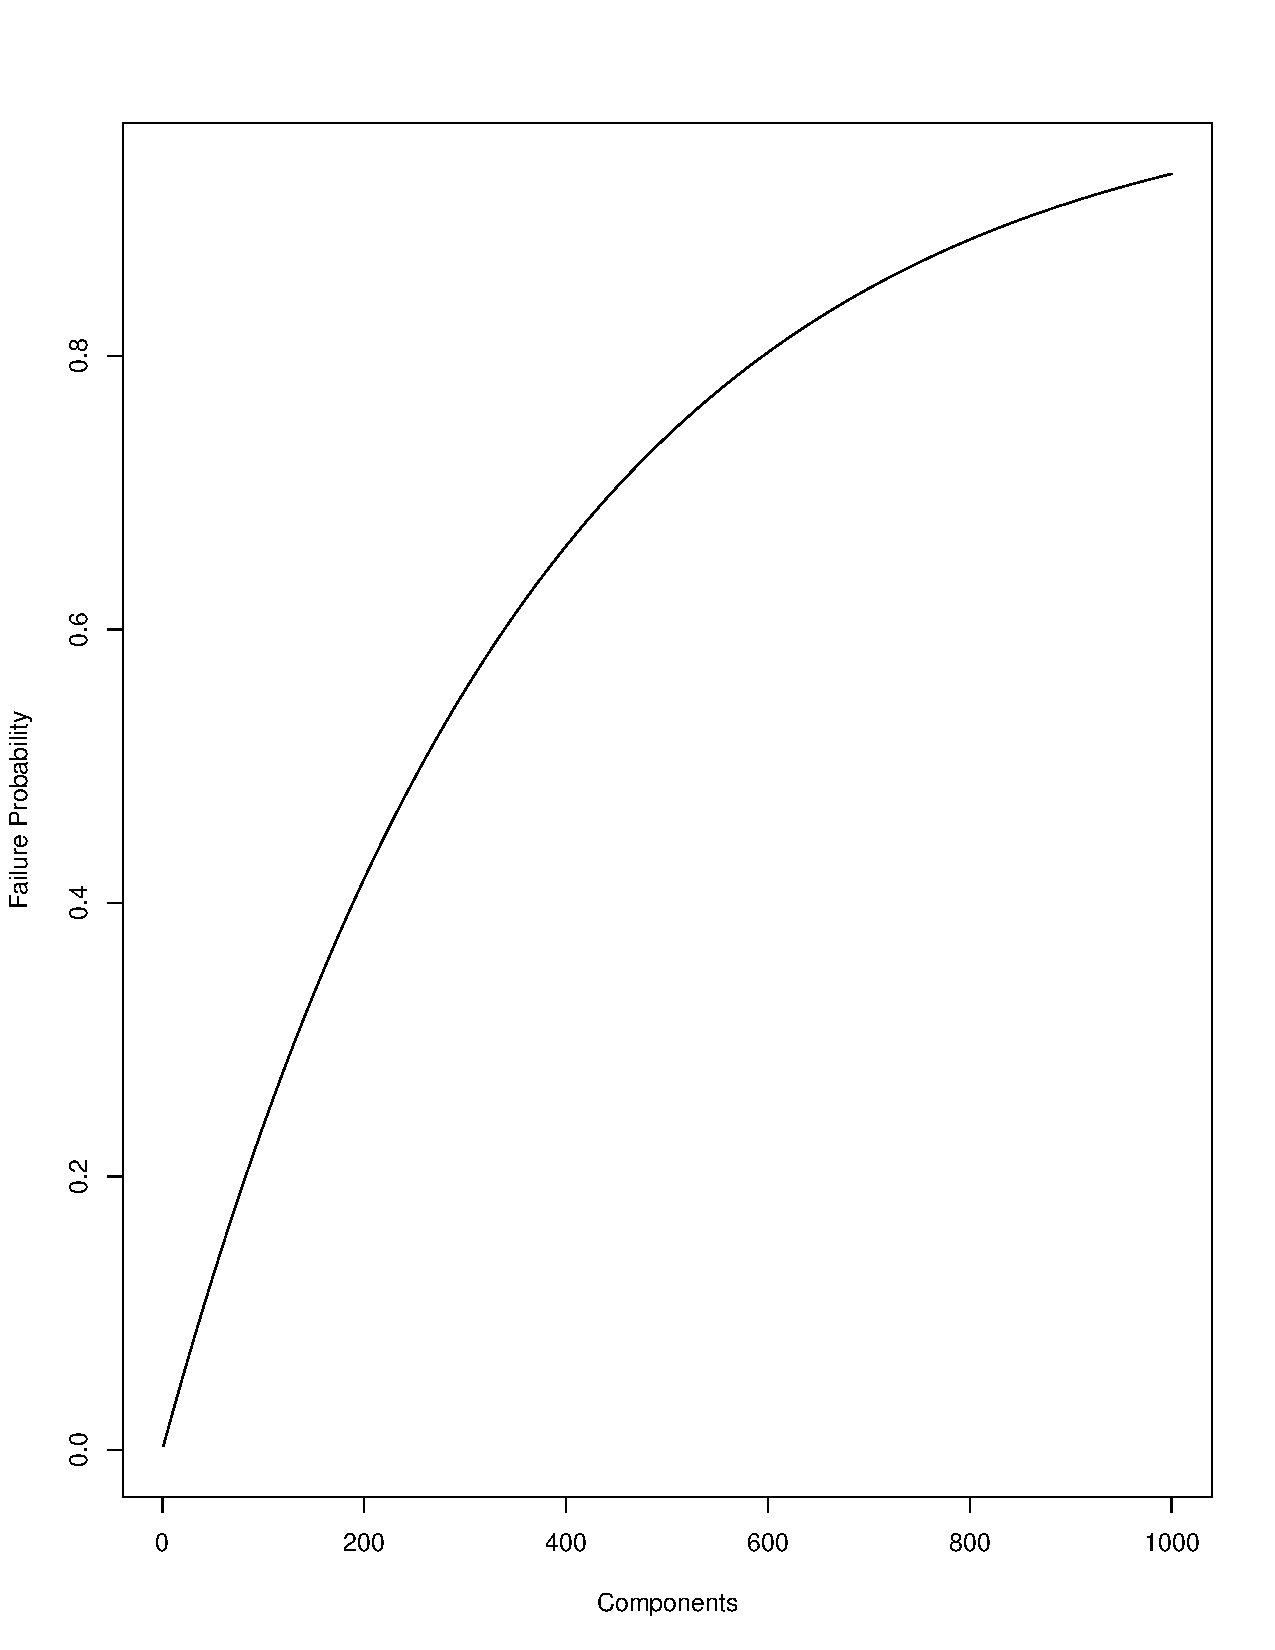
\includegraphics[width=0.8\linewidth]{art/faillure_probability}
\caption[3-sigma probability of failure]{\footnotesize 
	The probability of failure as a function of components under the 3-sigma standard.}
\label{fig:3_sigma_failure_proability}
\end{minipage}\hfill
\begin{minipage}{0.45\textwidth}
\centering
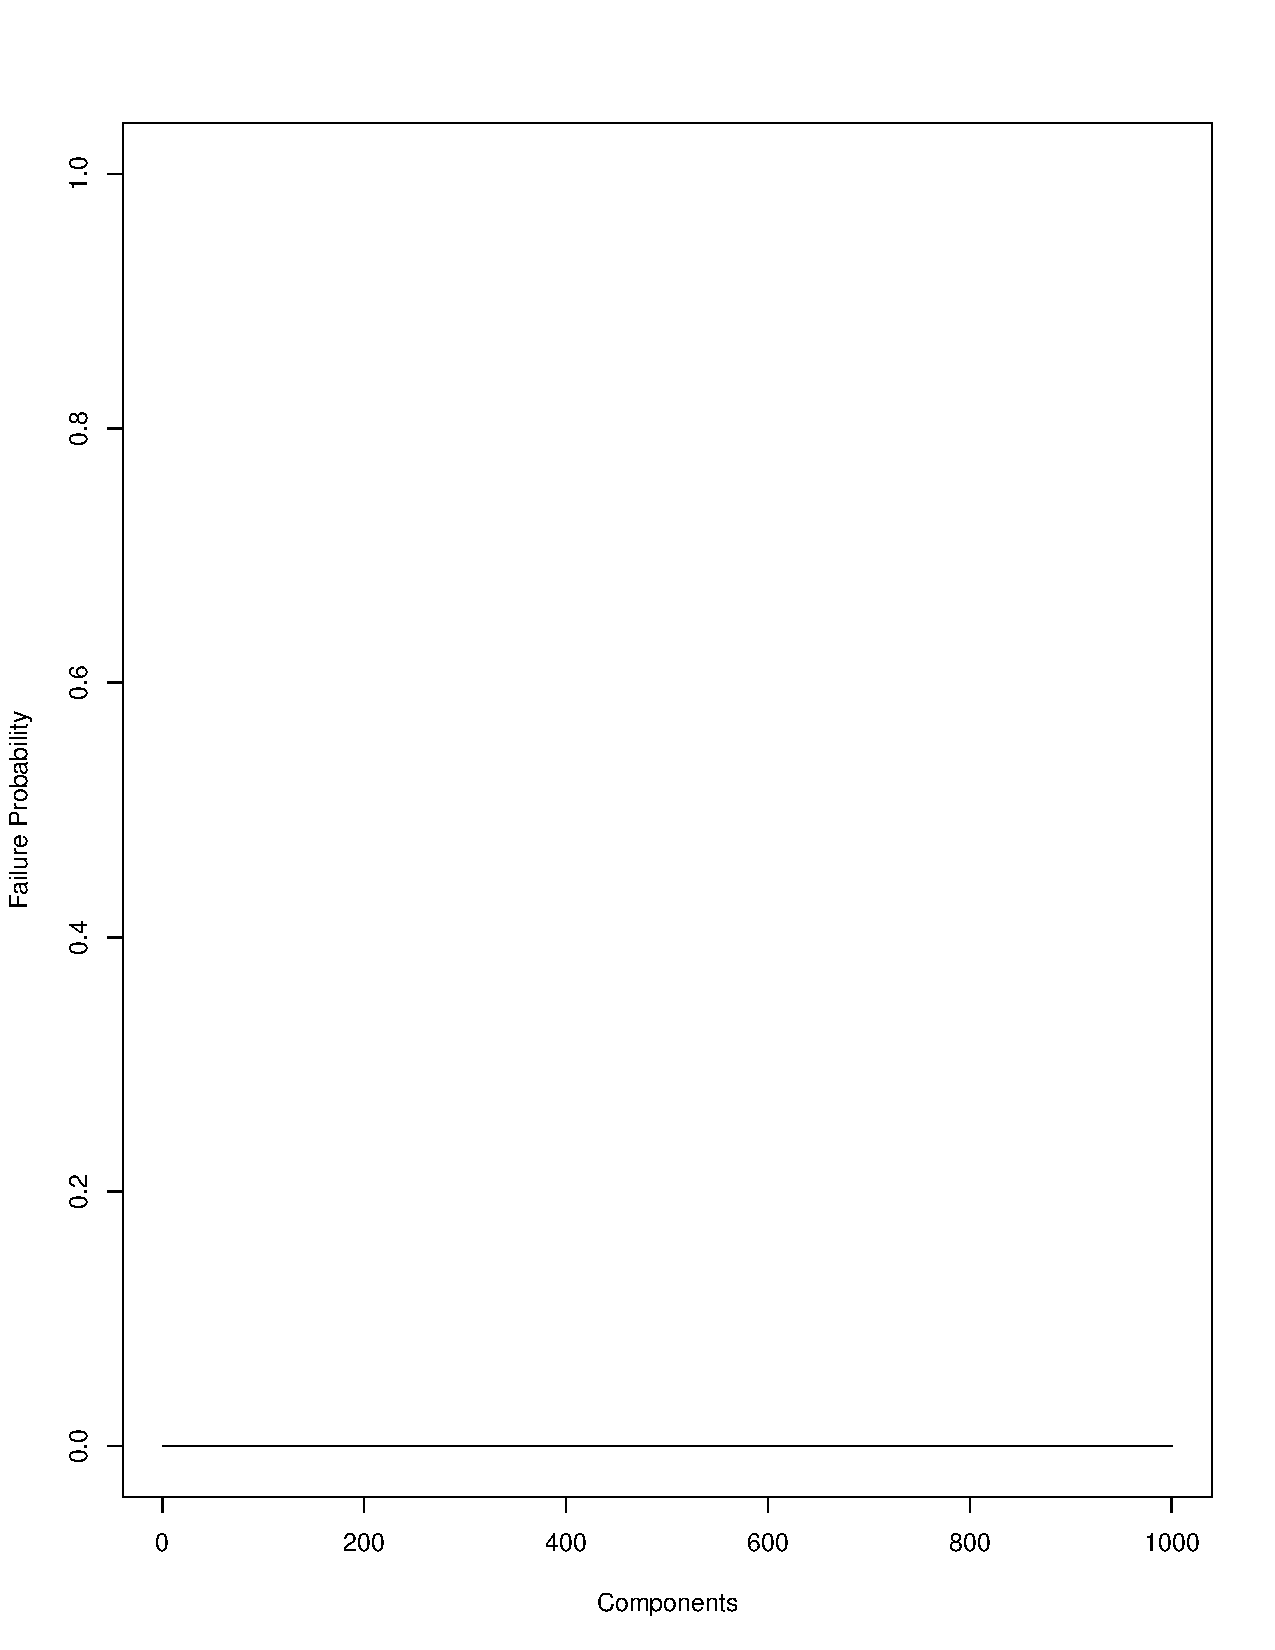
\includegraphics[width=0.8\linewidth]{art/6-sigma_failure_probability}
\caption[6-sigma probability of failure]{\footnotesize 
	The probability of failure as a function of components under the 6-sigma standard.}
\label{fig:6_sigma_failure_proability}
\end{minipage}
\end{figure}

According to \cite{montgomery_introduction_2007}, the 6-sigma methodology has gained more success than it predecessors:
\begin{quote}
The reason for the success of six-sigma in organizations outside the traditional manufacturing sphere is that variability is everywhere, and where there is variability, there is an opportunity to improve business results. 
\end{quote}



\subsection{Lean Systems}
Quoting \cite{wikipedia_lean_2015} (my own emphasis in bold):
\begin{quote}
Essentially, lean is centered on making obvious what \textbf{adds value} by \textbf{reducing everything else}. Lean manufacturing is a management philosophy derived mostly from the Toyota Production System (TPS) (hence the term Toyotism is also prevalent) and identified as ``lean'' only in the 1990s.
\end{quote}

\subsection{Design for Six-Sigma (DFSS)}
\label{sec:dfss}

Quoting \cite{wikipedia_design_2015} (my own emphasis in bold):
\begin{quote}
It is based on the use of \textbf{statistical tools} like linear regression and enables empirical research similar to that performed in other fields, such as social science. While the tools and order used in Six Sigma require a process to be in place and functioning, DFSS has the objective of \textbf{determining the needs of customers} and the business, and driving those needs into the product solution so created. DFSS is relevant for relatively simple items / systems. It is used for product or process design in contrast with process improvement.
\end{quote}




\subsection{Quality Systems and Standards}
The first quality standard was issued by the International Standards Organization (ISO) in $1987$.\marginnote{ISO9000}
Current quality standards are known as the \emph{ISO9000 series}. These include:
\begin{description}
\item [ISO9000:2000] Quality Management System-Fundamentals and Vocabulary.
\item [ISO9001:2000] Quality Management System-Requirements.
\item [ISO9004:2000] Quality Management System-Guidelines for Performance Improvement.
\end{description}
In Israel, it is the Standards Institute of Israel\footnote{\url{https://portal.sii.org.il/heb/qualityauth/certificationtypes/qualitylinks/iso9001/}} that may give ISO9000 (like any ISO) certifications upon inspecting the candidate organization.
As emphasized by \citet[p.24]{montgomery_introduction_2007}, ISO9000 is a set of rules and best practices, mostly oriented at \emph{knowledge management}. 
It may help to \emph{preserve} quality, but it does not, nor does it aim to, \emph{improve} quality.
As such, it will not be the focus of our course, which will focus on \emph{statistical tools}.


\begin{extra}

[TODO: Just-in-Time, Poka-Yoke]

\end{extra}




\section{DMAIC}
There are many names for the process of quantitative re-evaluations of performance against a given target: \emph{data driven decision making} (DDD), \emph{Shewart cycle}, etc.
We will focus on one such framework, illustrated in Figure~\ref{fig:DMAIC} known as DMAIC: Define, Measure, Analyze, Improve, Control.


\begin{figure}[t]
\centering
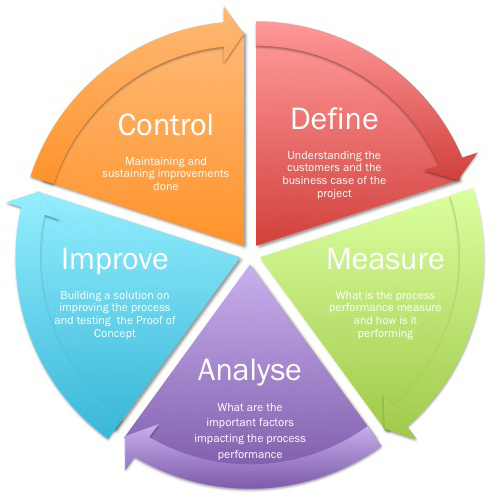
\includegraphics[width=0.6\linewidth]{art/Sigma_detail}
\caption[DMAIC]{The DMAIC cycle. \newline
\url{http://www.sapartners.com/sigma-academy/}}
\label{fig:DMAIC}
\end{figure}

Here are some general observations on DMAIC:
\begin{enumerate}
\item It is aimed at promoting improvement and creative thinking.
\item It is not part of the six-sigma methodology, but will typically take part in its implementation.
\end{enumerate}

What do the stages of DMAIC mean \footnote{\url{http://asq.org/learn-about-quality/six-sigma/overview/dmaic.html}}?
\begin{description}
\item [Define] the problem, improvement activity, opportunity for improvement, the project goals, and customer (internal and external) requirements.
\item [Measure] process performance.
\item [Analyze] the process to determine root causes of variation, poor performance (defects).
\item [Improve] process performance by addressing and eliminating the root causes.
\item [Control] the improved process and future process performance.
\end{description}

In the following chapter we give a set of statistical tools required for \emph{measuring},\emph{analyzing} and \emph{controlling} a process.